\documentclass[8pt]{beamer}
\usepackage{pdfpages}
\usepackage{graphicx}
\usepackage{float}
% \usepackage{subfig}
\usepackage{subfigure}
\usepackage{multirow}
\usepackage[ruled, linesnumbered]{algorithm2e}
\usepackage{pslatex}
\usepackage{amsmath}
% \usepackage[cm]{fullpage}
% \usepackage[margin=2.5cm]{geometry}
% \usepackage{lscape}

\newtheorem{objective}{Objective}
\newtheorem{methodology}{Methodology}
\newtheorem{motivation}{Motivation}
\newtheorem{advantage}{Advantages}
\newtheorem{method}{Method}
\newtheorem{question}{Possible Question}

% Class options include: notes, notesonly, handout, trans,
%                        hidesubsections, shadesubsections,
%                        inrow, blue, red, grey, brown
\usetheme{Madrid}
% Theme for beamer presentation.
% \usepackage{beamerthemesplit} 
% Other themes include: beamerthemebars, beamerthemelined, 
%                       beamerthemetree, beamerthemetreebars  

% Enter your title between curly braces
\title[Master Thesis Presentation]{Hybrid Acceleration for Interest-based \\ Contour Component Extraction}
\author{Liangfu Chen}                 % Enter your name between curly braces
\institute[V.R. Lab.]{School of Computer Science \& Engineering\\Chung-Ang University}      % Enter your institute name between curly braces
\date{\today}                    % Enter the date or \today between curly braces

\begin{document}

% Creates title page of slide show using above information
\begin{frame}
  \titlepage
\end{frame}
\note{}
% \note{Talk for 10 minutes} % Add notes to yourself that will be displayed when
                           % typeset with the notes or notesonly class options

% \section[Outline]{}

% Creates table of contents slide incorporating
% all \section and \subsection commands
% \begin{frame}{Outline}
%   \tableofcontents
% \end{frame}

% \section{Previous Works}

% \begin{frame}{Previous Works}
%   \frametitle{Simple slide with three points shown all at once}   % Insert frame title between curly braces

%   \begin{itemize}
%   \item Point 1
%   \item Point 2
%   \item Point 3
%   \end{itemize}
% \end{frame}
% \note[enumerate]       % Add notes to yourself that will be displayed when
% {                      % typeset with the notes or notesonly class options
% \item Note for Point 1   
% \item Note for Point 2   
% }


\begin{frame}
  \frametitle{Overview}
  \begin{objective}
    \structure{Improve the interaction of 3D volume data visualization}
  \end{objective}
  \begin{methodology}
    \structure{Region of Interest Computation}
    \begin{itemize}
    \item Contour tree is used as visual index of regions in volume
    \item Contour tree simplification reduce noisy contour structures
    \end{itemize}
    \structure{Parallel Contour Propagation}
    \begin{itemize}
    \item Use ``task-stealing'' method get seed cell in a thread
    \item Collect tetrahedral cell with intersection (to avoid visiting empty cell)
    \end{itemize}
    \structure{GPU-based Cell Triangulation}
    \begin{itemize}
    \item Predict size of triangle in mesh (parallel prefix sum)
    \item Render it directly (to prevent reading back to main memory)
    % \item Pack data small in size (to reduce data transfer to GPU)
    \end{itemize}
  \end{methodology}
\end{frame}
\note{
\underline{Contour tree is used as visual index of subregions in volume}
and these indices are provided 

}


\begin{frame}
  \frametitle{Motivation \& Advantage}
  % \begin{motivation}
  %   \begin{itemize}
  %   \item \structure{Region of Interest Computation}
  %     \begin{itemize}
  %     \item
  %     \end{itemize}
  %   \item \structure{Parallel Contour Propagation}
  %     \begin{itemize}
  %     \item Fast Isocontouring method -- a single seed for each
  %       contour
  %     \item Task stealing method for dequeue algorithm
  %     \end{itemize}
  %   \item \structure{GPU-based Triangulation}
  %     \begin{itemize}
  %     \item CUDA has been used for isosurface extraction
  %     \end{itemize}
  %   \end{itemize}
  % \end{motivation}

  \begin{advantage}
    \structure{Advantages of parallel contour propagation in CPU}
    \begin{itemize}
    \item Highly optimized for heavy conditional control operations\\
      $\rightarrow$ task-stealing algorithm is designed to avoid starvation
    \end{itemize}
    \structure{Advantages of triangulate active cells in GPU}
    \begin{itemize}
    \item GPGPU interoperable with rendering pipeline \\
      $\rightarrow$ render the surface without reading back to main
      memory
    \item Parallel computation pipeline \\
      $\rightarrow$ general purpose programming with less conditional control
    \end{itemize}
  \end{advantage}
\end{frame}
\note{}

% \begin{frame}
%   \frametitle{GPU versus CPU}
%   \begin{figure}[H]
%     \centering
%     \includegraphics[width=.7\textwidth]{images/gpu_vs_cpu.PNG}
%     \caption{GPU vs CPU}
%     \label{fig:gpu_vs_cpu}
%   \end{figure}
% \end{frame}

\section{Region of Interest Computation}

\begin{frame}
  \frametitle{Contour Tree}
  \begin{figure}[H]
    \centering
    \includegraphics[width=.8\textwidth]{images/contour_tree_hemoglobin.png}
    \caption{Contour Tree with mapped contours}
    % \label{fig:contree}
  \end{figure}
  \begin{itemize}
  \item \structure{contour tree edges:} monotone structure in volume
  \item \structure{contour tree nodes:} local maximum/minimum \& contour topological changes
  \end{itemize}
\end{frame}
\note{}

\begin{frame}
  \frametitle{Contour Tree Simplification}
  \begin{figure}[H]
    \centering
    \subfigure[coarse simplified 1]{\includegraphics[width=.3\textwidth]{images/contour_tree_simp0.png}}
    \subfigure[coarse simplified 2]{\includegraphics[width=.3\textwidth]{images/contour_tree_simp1.png}}
    \subfigure[fine simplified]{\includegraphics[width=.3\textwidth]{images/contour_tree_simp2.png}}
    \caption{Contour Tree Simplification (by persistence value)}
    % \label{fig:contree_simp}
  \end{figure}
\end{frame}
\note{}

\section{Parallel Contour Propagation}


\begin{frame}
  \frametitle{Task-stealing Method % for Dequeue Seed Cells in Threads
  }
  \begin{columns}
    \begin{column}{.5\textwidth}
      \begin{figure}[htb]
        \centering
        % \includegraphics[width=.6\textwidth]
        % {images/mt-engine-21.png}
        % \caption{Engine image data with color-tags for threads}
        \includegraphics[width=.8\textwidth]{images/drawing3}
        \caption{Conventional method}
      %   % \label{fig:engine}
      % \end{figure}
      % \begin{figure}[H]
      %   \centering
        \includegraphics[width=0.5\textwidth]{images/mt-sphere-propagate.png}
        \caption{parallel propagation}
      \end{figure}
    \end{column}
    \vline{}
    \begin{column}{.5\textwidth}
      \structure{conventional method}
      \begin{itemize}
      \item enqueue every intersected neighboring cells for further propagation
      \end{itemize}
      \structure{parallel propagation method}
      \begin{itemize}
      \item keep a local queue in each thread
      % \item steal a seed cell from the local queue in other threads
      \item steal a seed cell from other threads
      \item propagate till local queue is empty
      \end{itemize}
      \begin{question}
        \underline{Why not implement this algorithm in GPU?}\\
        \structure{Answer:}\\
        In short: due to the heavy conditional controls
        \begin{itemize}
        \item time consuming to fetch global memory in GPU
        \item time consuming to manage GPU threads
        \item different number of tasks assigned to GPU threads result in worst performance
        \end{itemize}
      \end{question}
    \end{column}
  \end{columns}
\end{frame}
\note{}

\begin{frame}
  \frametitle{Avoid Visiting Empty Cell -- Active Cells}
   \begin{columns}
    \begin{column}{0.5\textwidth}
      \begin{figure}[H]
        \centering
        \includegraphics[width=.7\textwidth]{images/activecell-activeblock.png}\\
        \caption{Collected Active Block in Volume}
        \includegraphics[width=.7\textwidth]{images/activecell-surface-fuel.png}
        \caption{Triangulated Surface Mesh}
        \label{fig:act_cell_tri}
      \end{figure}
    \end{column}
    \vline{}
    \begin{column}{0.5\textwidth}
      \begin{itemize}
      \item \structure{Active cell:} Tetrahedral cells with intersection to isovalue 
        that is interactively selected.\\
        $\rightarrow$ these cells are combined from all thread-specific arrays
      \end{itemize}
      \structure{Advantages}
      \begin{itemize}
      \item reduce data transfer to GPU\\ (depend on CPU to GPU bandwidth)
      \item reduce graphics card memory usage
      \end{itemize}
    \end{column}
  \end{columns}
  
\end{frame}
\note{}

\section{GPU-based Cell Triangulation}

\begin{frame}
  \frametitle{Parallel Prefix Sum}
  \structure{Parallel Prefix Sum}
  \begin{itemize}
  \item predict size of memory used in each thread
  \item preallocate GPU global memory before triangulation
  \item assign same amount of task to each GPU thread without collision
  \item map GPU array address to VBO ID for direct rendering
  \end{itemize}
  \begin{figure}[H]
    \centering
    \includegraphics[width=0.5\textwidth]{images/scan.pdf}
    \caption{Parallel Prefix Sum (each tetrahedral cell can be triangulated into 1$\sim$2 triangles)}
    % \label{fig:39fig10}
  \end{figure}
\end{frame}
\note
{
  Two arrays are copied into GPU global memory after we combine active cells in threads
  \begin{itemize}
  \item array with cell index
  \item array with parallel prefix sum (scan)
  \end{itemize}
  In the case showing on the slide, cell A correspond to position 1 to put triangulated mesh.

  And \textbf{B} for position \textbf{2}, \textbf{C} for position \textbf{4}, 
  \textbf{D} for position \textbf{6} respectively.

  The task executed in each GPU thread \textbf{won't conflict} with other threads.
  
  This would be \textbf{efficient} during GPU kernel execution.
}

\begin{frame}
  \frametitle{VBO-based Dynamic Drawing}
  \structure{The VBO (Vertex Buffer Object)} \\
  \begin{itemize}
  \item vertex attributes in high-performance memory
  \item promotes efficient data transfer
  \end{itemize}
  \begin{method}
    \begin{itemize}
    \item \structure{before kernel execution:} Map VBO IDs to address of CUDA
      variable addresses.
    \item \structure{after kernel execution:}
      \begin{enumerate}
      \item Unmap the addresses to VBO IDs 
      \item Bind the VBO with vertex array and normal array
      \end{enumerate}
    \end{itemize}
  \end{method}
  \begin{advantage}
    \begin{itemize}
    \item rendering with GPGPU results without reading back to main memory
    \item only update vertices that is changed (improve rendering efficiency)
    \end{itemize}
  \end{advantage}
\end{frame}
\note{}

% \begin{frame}
%   \frametitle{Pack data small in size}
  
% \end{frame}

% \begin{frame}
%   \begin{figure}[htb]
%     \centering
%     \includegraphics[width=.3\textwidth]
%     {images/mt-engine-21.png}
%     \includegraphics[width=.3\textwidth]
%     {images/mt-engine-22.png}
%     \includegraphics[width=.3\textwidth]
%     {images/mt-engine-23.png}
%     \caption[Engine image data with color-tags for threads]
%     {A contour component extracted from engine image data,
%       where color shows contribution of different processors.}
%     % TODO: figure out the NNNs
%     \label{fig:engine}
%   \end{figure}
% \end{frame}

\begin{frame}
  \frametitle{Estimate the number of threads use % to obtain best performance
  }
  \begin{figure}[h!]
    \centering
    \fbox{\includegraphics[width=\textwidth-2in]{images/fig-perf-plot.pdf}}
    \caption[Multi-threading Contour Propagation Performance]
    {Multi-threading contour propagation performance tested on hemoglobin data.
      % ($y$ axis shows time to obtain 1,237,574 tetrahedral cells, while
      % lines show fitting function: 
      % $f(x) = \frac{\alpha}{x^\beta + \beta x + \gamma} + \delta  arctan (\epsilon  x+\zeta)+\eta$
    }
    \label{fig:threading1}
  \end{figure}
\end{frame}
\note{}

% \begin{frame}
%   \frametitle{Active Cell Triangulation}

%   \begin{columns}
%     \begin{column}{0.5\textwidth}
%       \begin{figure}[H]
%         \centering
%         \includegraphics[width=.7\textwidth]{images/activecell-activeblock.png}\\
%         \caption{Collected Active Block in Volume}
%         \includegraphics[width=.7\textwidth]{images/activecell-surface-fuel.png}
%         \caption{Triangulated Surface Mesh}
%         \label{fig:act_cell_tri}
%       \end{figure}
%     \end{column}
%     \vline{}
%     \begin{column}{0.5\textwidth}
%       \begin{itemize}
%       \item Each tetrahedral cell can be triangulated into 1$\sim$2 triangles
%       \end{itemize}
%       What do we want to get?
%       \begin{itemize}
%       \item Allocation of GPU memory of all triangles
%         % \pause{}
%       \item Allocation of GPU memory of all triangles
%       \end{itemize}
%     \end{column}
%   \end{columns}
% \end{frame}
% \note[test test]{555555555555555}


\begin{frame}
  \frametitle{Performance Improvement}
  \begin{figure}[H]
    \centering
    \includegraphics[width=.7\textwidth]{images/fig-perf-bar.pdf}
    % \includegraphics[width=\textwidth/2]{images/fig-perf-bar.pdf}  
    \caption[Performance comparison with the original method]
    {A performance comparison between conventional sequential program and the 
      composed hybrid accelerated method. (saved \huge{76\%} \normalsize{of the time in average)}
      % (executed on Linux environment with a Intel E5300 and a Nvidia
      % GeForce 9500 GT graphics card)
    }
    \label{fig:_perf_bar}
  \end{figure}
  
\end{frame}
\note{}

\begin{frame}
  \frametitle{Final Results}
\begin{figure}[H]
  \centering
    \includegraphics[width=0.3\textwidth]{images/result2-fuel}
    \includegraphics[width=0.3\textwidth]{images/result2-hemoglobin}
    \includegraphics[width=0.3\textwidth]{images/result2-engine}\\
    \includegraphics[width=0.3\textwidth]{images/result2-vh4}
    \includegraphics[width=0.3\textwidth]{images/result2-kidney}
    \includegraphics[width=0.3\textwidth]{images/result2-head}
  \caption{Final results (alpha blending enabled for showing internal regions of interest)}
  \label{fig:result-img2}
\end{figure}
  
\end{frame}
\note{}

\newtheorem{conclusion}{Conclusion}
\newtheorem{futureworks}{Future Works}
\begin{frame}
  \frametitle{Conclusion and Future Works}
  \begin{conclusion}
    % \structure{Region of Interest Computation}
    % \begin{itemize}
    % \item
    % \end{itemize}
    \structure{Performance Improvement}
    \begin{itemize}
    \item The proposed algorithm guarantees at least 50\% of performance improvement on modern 
      computers with multi-core CPU(s) and many-core GPU(s).
    \end{itemize}
    \structure{Time complexity}
    \begin{itemize}
    \item Ideally, the proposed algorithm for propagating contours reduce the original $O(n)$ method 
      to $O(n/\alpha)$\\
      $\rightarrow$ \emph{n} stand for the size of contour, and $\alpha$ stand for the number 
      of cores exist in CPU(s).
    \end{itemize}
  \end{conclusion}
  \begin{futureworks}
    \begin{itemize}
    \item With surface mesh triangulated in GPU, it's easy to compute the property of the contour.\\
      $\rightarrow$ these properties can be useful for estimating important regions that people might be interested.
    \item Develop out-of-core method that can visualize larger surfaces without limitation of main memory 
      and GPU performance using proposed hybrid acceleration method.
    \end{itemize}
  \end{futureworks}
\end{frame}
\note{}

\begin{frame}{Q \& A}
  \begin{center}
    \Large{\structure{Questions and Answers}}\\
    \normalsize{\structure{Thank you for your attention}}
  \end{center}
\end{frame}



% \subsection{Simple slide with three points shown in succession}

% \begin{frame}
%   \frametitle{Simple slide with three points shown in succession}   % Insert frame title between curly braces

%   \begin{itemize}
%   \item<1-> Point 1 (Click ``Next Page'' to see Point 2) % Use Next Page to go to Point 2
%   \item<2-> Point 2  % Use Next Page to go to Point 3
%   \item<3-> Point 3
%   \end{itemize}
% \end{frame}
% \note{Speak clearly}  % Add notes to yourself that will be displayed when
% % typeset with the notes or notesonly class options


% \section{Slide with two columns: items and a graphic}

% \begin{frame}
%   \frametitle{Slide with two columns: items and a graphic}   % Insert frame title between curly braces
%   \begin{columns}[c]
%     \column{2in}  % slides are 3in high by 5in wide
%     \begin{itemize}
%     \item<1-> First item
%     \item<2-> Second item
%     \item<3-> ...
%     \end{itemize}
%     \column{2in}
%     \framebox{Insert graphic here % e.g. \includegraphics[height=2.65in]{graphic}
%     }
%   \end{columns}
% \end{frame}
% \note{The end}       % Add notes to yourself that will be displayed when
% % typeset with the notes or notesonly class options

\end{document}
